\documentclass[10pt,letterpaper,twocolumn,twoside,fleqn]{article}
\usepackage[utf8]{inputenc}
\usepackage{amssymb}
\usepackage[left=1.69cm,right=1.69cm,top=2.2cm,bottom=2.2cm,footskip=0.5cm,headsep=0.5cm]{geometry}
\usepackage{color}
\definecolor{TRED}{RGB}{192, 0, 0}
\definecolor{Tgray}{RGB}{160, 160, 160}
\usepackage{multicol}
\usepackage{times}
\usepackage{here} 
%% ----- Papers en Español  ------
%% Descomentar estas líneas para documentos en español
\usepackage[spanish]{babel} 
\usepackage[font={footnotesize},labelfont={footnotesize},justification=centering,figurename=Figura,tablename=Tabla]{caption}
% %----- Papers en Español  ------


%% ---- English Papers ---------
% %uncomment this lines for english papers
%\usepackage[english]{babel}
%\usepackage[font={footnotesize},labelfont={footnotesize},justification=centering,figurename=Figure,tablename=Table]{caption}
%% ---- English Papers ---------





\usepackage[protrusion=true,expansion=true]{microtype} 
\usepackage{amsmath,amsfonts,amsthm}
\usepackage[svgnames]{xcolor} 
\usepackage{fix-cm}	
\usepackage{graphicx} 
\usepackage{multirow}
\usepackage{titlesec}
\usepackage{setspace}
\usepackage[labelfont=bf]{caption}

%%%%%%%%%%%%%%%%%%%%%%%%%%%%%%%%%%%%%%%%%%%%%%%%%%%%%%%%%%%%%
%%%% Formato Titulo de Sección - No modificar %%%%%%%%%%%%%%%
%%%%%%%%%%%%%%%%%%%%%%%%%%%%%%%%%%%%%%%%%%%%%%%%%%%%%%%%%%%%%

\titleformat{\section}
  {\fontsize{11}{11}\selectfont \bfseries}{\thesection}{0.3em}{}
  
\titleformat{\subsection}
  {\normalfont \itshape}{\thesubsection}{0.3em}{}[\vspace*{-0.2cm}]

\titleformat{\subsubsection}
  {\normalfont \itshape}{\thesubsubsection}{0.3em}{}[\vspace*{-0.2cm}]
  
%%%%%%%%%%%%%%%%%%%%%%%%%%%%%%%%%%%%%%%%%%%%%%%%%%%%%%%%%%%%%
%%%% Formato Encabezado y pie de página     %%%%%%%%%%%%%%%%%
%%%%%%%%%%%%%%%%%%%%%%%%%%%%%%%%%%%%%%%%%%%%%%%%%%%%%%%%%%%%%

\usepackage{fancyhdr} 
\fancypagestyle{plain}
{
\fancyhf{}
\renewcommand{\headrulewidth}{0pt}
\fancyhead[C]{{\textcolor{Tgray}{\textit{{\textbf{BISTUA} Rev. FCB, Volumen 20 (1) (2022), 1-15. Pamplona -Colombia }}}}
\vspace*{0cm}
\begin{picture}(0,0) \put(-390,-96)
{
\includegraphics[width=17.51cm]{Encabezadoarticulo_2.png} }
\end{picture}}
\fancyfoot[L]{
\hline
\vspace{0.3cm}
\setlength{\parindent}{0.05cm}{{\footnotesize © \textit{\textcolor{Tgray}{Autores; Licencia Universidad de Pamplona
\includegraphics[scale=0.3]{cc_bistua_grande.png}\hspace{5.4cm} 
%% INSERTE AQUÍ EL %DOI
https://doi.org/10.24054/01204211.v18.n1.2020.xxxx
%%% FIN DOI
}} \\\vspace{-0.1cm}  }}
}


				}
\renewcommand{\headrulewidth}{0pt}
\renewcommand{\footrulewidth}{0pt}
					}

\fancyhf{}
\rhead[{\footnotesize \textit{\textcolor{Tgray}{BISTUA Rev. FCB, Vol. 20 (1), (2022)}}}]{{\footnotesize \textit{\textcolor{Tgray}{BISTUA Rev. FCB, Vol. 20 (1), (2022)}}}}
\rfoot[]{}
\lfoot[]{}
\cfoot[\thepage]{\thepage}
\renewcommand{\headrulewidth}{1.5pt}
\renewcommand{\headrule}{\hbox to\headwidth{%
  \color{Tgray}\leaders\hrule height \headrulewidth\hfill}}
\renewcommand{\footrulewidth}{0pt}
\pagestyle{fancy}


%%%%%%%%%%%%%%%%%%%%%%%%%%%%%%%%%%%%%%%%%%%%%%%%
%%%%%%%%%%%% Formato de Titulo %%%%%%%%%%%%%%%%%
%%%%%%%%%%%%%%%%%%%%%%%%%%%%%%%%%%%%%%%%%%%%%%%%

\usepackage{titling} 
\pretitle{\vspace{30pt} \begin{flushleft} \setlength{\parindent}{0.5cm} \fontsize{16}{32}\selectfont \bfseries  } 

%________________________________________
%INSERTAR TITULO AQUI:
	\title{ 
	\vspace{0.5cm}
	\hspace{0.3cm} 
	Plantilla de Autor: Instrucción para preparación del manuscrito\\
	 \vspace*{-0.7cm}{\small \textit{Author Template: Instruction for preparation of manuscript}}}
%________________________________________

\posttitle{\par\end{flushleft}} 

\preauthor{ \begin{flushleft} \lineskip 0.4em \fontsize{10}{14}\selectfont   }  % Author font configuration

%_________________________________________
% INSERTAR AUTORES AQUI:
 	\author{\hspace{0.38cm} \textbf{Nombre 1 (s) Apellido 1 (s)}$^{a}$;    \textbf{Nombre 2 (s) Apellido 2 (s)}$^{b}$; \textbf{Nombre 3 (s) Apellido 3 (s)}$^{b}$ }	
%__________________________________________

\postauthor{\lineskip 0.5em  \setlength{\parindent}{0.5cm} \fontsize{10}{10}\selectfont % 
\\ \vspace{0.4cm}

%________________________________________
% INSERTAR INSTITUCIONES AQUI:
{\small $^{a}$ \textit{Datos filiación institucional, País} \\
$^{b}$ \textit{Datos filiación institucional, País}}
 %_______________________________________
 
 
 \vspace{0.3cm}
  % INSERTAR CORRESPONDENCIA AQUÍ:
 
 
 {\hspace{-0.3cm}\footnotesize
 \textit{\textbf{Correspondencia:} autorresponsable@unipamplona.edu.co}
 
 }
 
 
\vspace*{-0.3cm} 
\par\end{flushleft}} %
\predate{\begin{flushright} \fontsize{7.5}{7.5}\selectfont}
	\date{\textit{\textbf{Recibido}: Agosto 6, 2020. \hspace{0.15cm}\textbf{Aceptado}: Noviembre 04,2020.  \hspace{0.15cm}\textbf{Publicado}: Diciembre 12, 2020}}

	
\postdate{\par\end{flushright}}
%%%%%%%%%%%%%%%%%%%%%%%%%%%%%%%%%%%%%%%%%%%%%%%%%%%%%%%%%%%%%%%%%%%%%%%%%%%%%%%%%%%%%
\begin{document}

\twocolumn[
	\maketitle
    \begin{@twocolumnfalse}  
	\vspace*{-1.4cm}
	\begin{center}
	 %\color{Tgray}{\rule{0.94\textwidth}{1.5pt}}
	\end{center}
	\vspace*{-0.55cm}
    %\hspace{0.6cm} %{\fontsize{9}{\baselineskip}\selectfon%t  https://doi.org/10.24054/01204211.v%18.n1.2020.xxxxv}
	%\\\\
	\begin{tabular}{p{8.7cm}p{8.7cm}}
	
	\hline
	\\
	
	
\setlength{\parindent}{0.0cm}{\textbf{Resumen}}  & \setlength{\parindent}{0.0cm}{\textbf{Abstract:} }
	\\ % EL RESUMEN SE ESCRIBE DESPUES DE LAS INSTRUCCIONES DE FORMATO 
\setlength{\parindent}{0.0cm}{	{\fontsize{9}{\baselineskip}\selectfont 
Este instructivo es una guía de pautas para preparar el manuscrito de artículos para BISTUA. Use este documento como plantilla en \LaTeX{} . El manuscrito debe estar escrito en español o inglés. La longitud del manuscrito no debe superar 7 páginas. Se debe mantener la totalidad del estilo de esta plantilla. El estilo de tipo de letra de la totalidad del manuscrito es Times New Roman; note que en cada aparte del manuscrito hay cambios en el tamaño y formato del texto (negrilla y cursiva). Por ejemplo, el título tiene tamaño 16, negrilla, alineación izquierda. Este resumen tiene la palabra Resumen en negrilla, tamaño 9. La longitud máxima del resumen no debe exceder 300 palabras. Las palabras clave están separadas por un punto y coma.
 	}
 		}
	  &
\setlength{\parindent}{0.0cm}{	{\fontsize{9}{0}\selectfont 
This instruction gives you guidelines for preparing papers for BISTUA. Use this document as a template in \LaTeX{}. The manuscript must be written in Spanish or English. The length of the manuscript should be kept within 7 pages. The entire style of this template must be maintained. The font style of the entire manuscript is Times New Roman; Note that in each part of the manuscript there are changes in the size and format of the text (bold and italic). For example, the title is size 16, bold, left aligned. This abstract has the word Abstract in bold, size 9. The maximum length of the abstract should not exceed 300 words. Keywords are separated by a semicolon. 
	}
		}
	\\\\
	\setlength{\parindent}{0.0cm}{\textbf{\textit{Palabras clave:}} formato del manuscrito; Instrucciones.
	} &
	\setlength{\parindent}{0.0cm}{\textbf{\textit{ Keywords:}} manuscript formatting; Instructions.
	}
	\\
	\hline
	\end{tabular}
		\vspace*{1cm}
 		\end{@twocolumnfalse}
]


\section{Preparación del manuscrito}\setlength{\parindent}{0cm}
El manuscrito presentado debe prepararse estrictamente de acuerdo con las pautas presentadas en este documento plantilla. Aceptamos el documento en editores de texto MS Word (97 o superior) o Latex siempre que conserve las características de esta plantilla. El texto del manuscrito debe escribirse dentro del área de 2159 mm x 2794 mm (tamaño carta estándar). Los márgenes son los que tiene esta plantilla. El documento debe escribirse a espacio simple utilizando la fuente Times New Roman, conservando los tamaños de letra establecidos en esta plantilla. Por ejemplo, el texto del cuerpo del artículo debe ser de 10 puntos, el título debe ser de 16 puntos; el resumen, los títulos de las figuras y las referencias deben ser de 8 puntos. Todos los títulos deben conservar el tamaño y estilo como aparece en esta plantilla.
\\\\
El título principal del artículo debe escribirse en minúsculas, centrado y en tamaño 16 puntos; el título traducción del principal debe ir centrado y en tamaño 11 puntos. Si el idioma principal del manuscrito es inglés, entonces el título principal debe ir en inglés y el título traducción en español, y viceversa. Utilice caracteres de superíndice para hacer referencia a los nombres de las afiliaciones de los autores, que deben escribirse en letra cursiva después de los nombres de los autores. Indique también la dirección de correo electrónico del autor responsable de la correspondencia. En general, para un artículo completo, el cuerpo del trabajo deberá contener la siguiente estructura: Introducción, Método y materiales, Resultados, Discusión y Conclusiones. 
\vspace*{-0.1cm}
\subsection{Amplitud y categorías de publicación}
Se recomienda la extensión del manuscrita no exceda 15 páginas. BISTUA acepta para publicación las siguientes modalidades:
\subsubsection{Artículo original}
Es un trabajo inédito derivado de una investigación que aporta información nueva sobre aspectos específicos y contribuye de manera relevante al conocimiento científico.
\subsubsection{Comunicación breve}
Es el informe de resultados parciales de una investigación cuya divulgación rápida es de gran importancia. Es un trabajo de 1.000 palabras, máximo, con un número de figuras y tablas no mayor de 2 y cuyo resumen no debe pasar de 100 palabras.\\
Los métodos, resultados y discusión se presentan agrupados en una única sección.
\subsubsection{Nota técnica}
Es un escrito breve en el que se describe en detalle una técnica de laboratorio novedosa o modificaciones realizadas a una técnica ya establecida, enfatizando las ventajas que tiene el procedimiento o la innovación desarrollada.
\subsubsection{Revisión de tema}
 Es un trabajo que constituye un ``estado del arte'' y que es presentado por expertos en un tema particular de las ciencias básicas, y que son invitados por el Comité Editorial. Se podrán someter en esta modalidad los trabajos de tesis de grado producto de una investigación.
\subsubsection{Números especiales } 
BISTUA podrá publicar números especiales de trabajos presentados en eventos de divulgación de resultados de investigación. En todo caso, las contribuciones deberán surtir el procedimiento de arbitraje establecido por BISTUA.
\subsubsection{Presentación de casos } 
Descripción de un cuadro clínico que destaca alguna particularidad llamativa o especial, con análisis amplio de la literatura pertinente.
\subsubsection{Cartas al editor} 
 Los lectores solicitan aclaraciones o presentan comentarios sobre cualquier material publicado en la revista. Todo material propuesto para publicación en Bistua, será revisado por el Comité Editorial y enviado para evaluación a evaluadores o pares científicos. Los editores informarán a los autores sobre la recepción de los trabajos, sobre los comentarios de los evaluadores y sobre la decisión final que se tome para su publicación. La revista Bistua se reserva el derecho de aceptar o rechazar los artículos y podrá hacer sugerencias que tiendan a mejorar su presentación. Los originales de los artículos permanecerán en los archivos de la revista hasta por un año.

\section{Edición de tablas y figuras}

\begin{figure}[H]
\centering
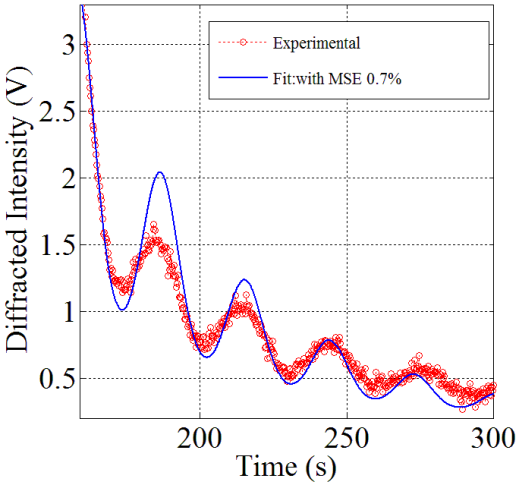
\includegraphics[width=4.62cm]{GraficaEjemplo.png} 
\caption{Ejemplo de presentación de resultados.\\
Fuente: [1]  ó  Fuente: Autor(es).}
\label{figura_1}
\end{figure}


Las figuras y tablas ocupan máximo el ancho de la columna; Use figuras y tablas de dos columnas de ancho solo si es absolutamente necesario.  Las tablas tienen el título encima de la tabla y las figuras tienen el título de debajo de ella (ver ejemplo Tab.\ref{tabla_1} y Fig.\ref{figura_1}). 

Todas las tablas y figuras se numeran consecutivamente con números arábigos. Vea un ejemplo de formato correcto de tablas y figuras en la Tab.\ref{tabla_1} y la Fig. \ref{figura_1}. Ubique las tablas y figuras cerca de la primera referencia a ellas, preferiblemente al principio o al final de cada columna. No use abreviaturas en los encabezados de columna. Para los subtítulos de tablas y figuras, y el texto en tablas, use la fuente Times New Roman con un tamaño de 8 puntos. Use solo líneas horizontales. Evite el texto en negrita. Las imágenes deben ser de alta calidad.


\begin{table}[H]
\centering
\caption{Ejemplo de tabla de datos.}
\begin{tabular}{ p{2.5cm} p{2.5cm} p{2.5cm}}
\hline 
Material & Temperatura  & Deformación \\ 
 & (°C)  & (mm) \\ 
\hline 
Plástico 1 & 61.08 & 8.06 \\
Plástico 2 & 61.93 & 6.16 \\ 
 - & - & - & \\
- & - & - & \\
- & - & - & \\ 
\hline 
\end{tabular} 
\label{tabla_1}
\end{table}

\section{Edición de ecuaciones}
Todas las ecuaciones deben estar numeradas consecutivamente y alineadas al margen izquierdo (ver Ec.\eqref{ecuacion_1}).


\begin{equation}
f(T)=\frac{1}{\sigma \sqrt{2 \pi}} \exp \left[-\frac{1}{2} \left( \frac{T-\mu}{\sigma}\right)^{2} \right]
\label{ecuacion_1}
\end{equation}

Use el editor de ecuaciones provisto por Microsoft Word o de \LaTeX{}. Use la convención estándar para la composición tipográfica de las matemáticas: letras en cursiva para variables escalares y constantes, letras en negrita en minúsculas para vectores y letras en negrita en mayúsculas para matrices. Por ejemplo, todas las variables en la Ec.\eqref{ecuacion_1} son escalares.

\section{Citación de bibliografía, tablas, figuras y ecuaciones}
Todas las referencias deben estar citadas en el texto del manuscrito; las referencias bibliográficas se deben citar de la siguiente forma: [1,2] o [1-3].  Para citar las figuras use Fig.1 o Fig.1-5, o Fig.1, 3 y 7. Para citar ecuaciones use Ec.(1) o Ec.(1)-(5).  La sección “Referencias” contiene ejemplos de la forma de como incluir los diferentes tipos de referencias bibliográficas: Artículos de revistas, Libros, Capítulos de libro, Artículos de memorias de eventos, Tesis.
\section{Conclusiones}

Presente aquí las conclusiones principales del trabajo. Comente los resultados relevantes del estudio, resaltando los aspectos nuevos e importantes. Puede exponer opiniones propias fundamentadas sobre los resultados y las consecuencias derivadas de la investigación, así como las limitaciones del estudio podrían ser comentadas. 



\section*{Reconocimientos}
\vspace{-0.3cm}
Es opcional. Aquí los autores pueden referir un reconocimiento a entidades que facilitaron o financiaron la investigación.



\begin{footnotesize}
\begin{thebibliography}{4}
\bibitem{R1} Maxwell J.C., A dynamical theory of the electromagnetic field, Philosophical Transactions of the Royal Society London 155 (1865) 459-512
\bibitem{R2} Restrepo G., Los elementos químicos, su matemática y relación con el sistema periódico. BISTUA Rev. FCB 2(1) (2004) 91-98. https://doi.org/10.24054/01204211.v1.n1.2004.17
\bibitem{R3} Salazar A., Rueda J.E., Study of energy coupling in a Bi12SiO20 photorefactive material, BISTUA Rev. FCB 2(1) (2004) 47-53. https://doi.org/10.24054/01204211.v1.n1.2004.11
\bibitem{R4} Tebaldi M.C., Rueda J.E, Bolognini N., Talbot interferometer based on a birefringence grating, Optics Communications 185(1) (2000) 65-76, doi: 10.1016/S0030-4018(00)00988-3
\bibitem{R5} Murcia R. M. A. Dynamic of the litterfall in a successional gradient of high andean forest of Colombia. Revista Bistua 17(3) (2019) 179-186.
https://doi.org/10.24054/01204211.v3.n3.2019.3576
\bibitem{R6} Masters T., Neural Network Recipes in C++. New York: Academic Press, 1993.

\bibitem{R7} Dvorak R., Ferraz-Mello, S., Eds., A Comparison of the dynamical evolution of planetary systems, Austria, Springer, 2004. http://dx.doi.org/10.1007/1-4020-4466-6$\#$sthash.TMeZ8aSQ.dpuf

\bibitem{R8} Moyor M.A., Evaluación del lenguaje de ingeniería, en Verdugo – Alonso J. Evaluación curricular: una guía para la intervención del ingeniero, 2a ed., Madrid, Salvat, 1994. pp. 324-344.

\bibitem{R9} Hoyles C., Noss R., What can digital technologies take from and bring to research in mathematics education? in Bishop, A.J. et al. Second International Handbook of Mathematics Education, 2nd edition, Dordrecht, Kluwer Academic, 2003, pp. 323-349.  http://dx.doi.org/10.1007/978-94-010-0273-8-11

\bibitem{R10} Jeng J.T., Chuang C.C., Chuang, C.-T., Support vector regression based LTS-CPBUM neural networks, Proceedings of SICE Annual Conference (SICE), 2011. pp. 215-220. 

\bibitem{R11} Kawasaki, N. Parametric study of thermal and chemical nonequilibrium nozzle flow, MSc. Thesis, Department of Electronic Engineering, Osaka University, Osaka, Japan, 1993.

\bibitem{R12} Williams, J. O. Narrow-band analyzer, PhD dissertation, Department of Electrical Engineering, Harvard University, Cambridge, MA, 1993.

\end{thebibliography}
\end{footnotesize}

%\bibliographystyle{ieeetr}
%\bibliography{bibliografia}}


\end{document}